\documentclass[10pt]{article}

\usepackage[utf8]{inputenc}
\usepackage[T2A]{fontenc}
\usepackage[russian, english]{babel}

\usepackage{amssymb, amsmath, textcomp, tabularx, graphicx}

\newcolumntype{C}{>{\centering\arraybackslash}X}%

\title{Задание 5}
\author{Коновалов Андрей, 074}
\date{}

\let \eps \varepsilon

\begin{document}

\maketitle

\noindent
\begin{tabularx}{\textwidth}{|C|C|C|C|C|C|C|}
  \hline
  0 & 1 & 2 & 3 & 4 & 5 & $\sigma$ \\
  \hline
  &&&&&& \\
  \hline
\end{tabularx}

\bigskip

{\bf Задача 1}

{\bf (i).} Допустим, что грамматика $G_1$ не однозначная. Это означает, что существует выводимое в $G$ слово, имеющее хотя бы 2 правых вывода.

Обозначим последовательности применения правил вывода для этих выводов $A$ и $B$ соответственно. Элементами этих последовательностей являются правила вывода.

Заметим, что $A$ и $B$ не могут содержать одна другую как префиксную подпоследовательность, значит существует такое $n \in \mathbb{N}$, что $A_n \neq B_n$.

Посмотрим на первое отличие в их выводах. Поскольку правил вывода всего 2, это означает, что в одном случае было применено правило $P_1 = S \rightarrow a$, а в другом правило $P_2 = S \rightarrow SSSb$. Поскольку выводы правые, то перед использованием $P_1$ и $P_2$ после которых слова становятся различными, слова имели вид: $xSy$, где $x \in \{ a, b, S \}^*$, $y \in \{ a, b \}^*$. После использования правила $P_1$ слово будет иметь суффикс $ay$, который не изменится после применения дальнейших правил вывода. После использования правила $P_2$ слово будет иметь суффикс $by$, который не изменится после применения дальнейших правил вывода. Заметим, что слова, получаемые выводами $A$ и $B$ не могут совпадать, поскольку имеют различные суффиксы.

Получаем противоречие, а значит выводов не может быть 2, а значит $G$ однозначная.

\smallskip

{\bf (ii).} Поскольку язык порождается некоторой праволинейной грамматикой тогда и только тогда, когда он регулярный, то доказав, что $L(G_1)$ - не регулярный, мы докажем, что $\nexists$ праволинейной грамматики эквивалентной $G_1$.

\smallskip

Для начала докажем, что на при любом выводе во любом получаемом промежуточном или конечном слове $x$ выполняется: $|x|_S + |x|_a = 2|x|_b + 1$. 

Заметим, что если в выводе сначала применить все правила вывода вида $P_2$, а потом - вида $P_1$, то выведенное слово не изменится. При применении правила $P_1$ количество букв $S$ уменьшается на 1, а количество букв $a$ увеличивается на 1, при этом соотношение остается верным. Это означает, что утверждение достаточно доказать для применения только правила $P_2$.

Заметим, что слова, получаемые при выводе имеют длину $n$, представимую ввиде $n = 3k + 1$, где $k$ - количество применений правила $P_2$. Докажем выполнимость соотношения индукцией по $k$.

{\it База.} При $k = 0$ существует единственное слово $S$ для которого соотношение выполняется. База доказана.

{\it Переход.} Пусть соотношение выполняется для количества применений $P_2$, которое $< k$. Слово $w$, получаемое применением $k$ применениями правила $P_2$, получено из слова $x$ применением правила $P_2$. Для $x$ верно $|x|_S + |x|_a = 2|x|_b + 1$. Заметим, что $|w|_S = |x|_S - 1 + 3 = |x|_S + 2$, $|w|_b = |x|_b + 1$, а значит $|x|_S + |x|_a = 2|x|_b + 1 \Leftrightarrow |x|_S - 2 + |x|_a = 2(|x|_b - 1) + 1 \Leftrightarrow |w|_S + |w|_a = 2|w|_b + 1$. Переход доказан.

\smallskip

Заметим, что в любом слове $w$ выводимом в $G$ не содержится нетерминал $S$, а значит $|w|_a = 2|w|_b + 1$.

Докажем, что язык $L(G_1)$ не регулярный пользуясь леммой о разрастании. Для любого $C$, возьмем слово $w = a^{2C + 1} b^{C}$, $|w| \geq C$. Для любого его разбиения $xyz$, такого, что $|xy| \leq C$ и $|y| > 0$, для $i = 2$ в слове $x y^i z$ нарушится соотношение между буквами $a$ и $b$, а значит $x y^i z \notin L(G_1)$.

Получаем, что лемма не выполняется, а значит $L(G_1)$ - не регулярный, а значит невозможно построить эквивалентную праволинейную грамматику.

\medskip

{\bf Задача 2}

{\bf (i).} Приведем два правых вывода одного слова:

$$S \rightarrow ict \; S \rightarrow ict \; ict \; S \; e \; S \rightarrow ict \; ict \; S \; e \; o \rightarrow ict \; ict \; o \; e \; o$$
$$S \rightarrow ict \; S \; e \; S \rightarrow ict \; S \; e \; o \rightarrow ict \; ict \; S \; e \; o \rightarrow ict \; ict \; o \; e \; o$$

\smallskip

{\bf (iii).} $G_3$ не однозначная, так существует два различных правых вывода слова $o$.

$$S \rightarrow S_1 \rightarrow o$$
$$S \rightarrow S_{full} \rightarrow o$$

\medskip

{\bf Задача 3}

Докажем, что следующие правила вывода порождают язык ППСВ $L_{3}$ с глубиной вложения скобок $\leq 3$. Аксиома $S_3$.
\begin{align*}
  S_0 &\rightarrow \eps \\
  S_1 &\rightarrow S_1 S_1 \\
  S_1 &\rightarrow ( S_0 ) \\
  S_1 &\rightarrow S_0 \\
  S_2 &\rightarrow S_2 S_2 \\
  S_2 &\rightarrow ( S_1 ) \\
  S_2 &\rightarrow S_1 \\
  S_3 &\rightarrow S_3 S_3 \\
  S_3 &\rightarrow ( S_2 ) \\
  S_3 &\rightarrow S_2 \\
\end{align*}

Будем называть правильные скобочные выражения с глубиной вложения скобок $i$ - ПСВ$_i$.

По индукции покажем, что нетерминал $S_i$ порождает ПСВ$_{\leq i}$. База индукции для $i = 0$ очевидна. Использование любого из правил ниже сохраняет правильность выражения. При использовании первого глубина вложений остается равной $i$. При использовании второго она увеличивается на 1 по сравнению с $i - 1$, т.е равна $i$. При использовании третьего она не изменяется, т.е. остается равной $i - 1$, что нас устраивает.
\begin{align*}
  S_i &\rightarrow S_i S_i \\
  S_i &\rightarrow ( S_{i - 1} ) \\
  S_i &\rightarrow S_{i - 1} \\
\end{align*}

Получаем, что $L(G) \subseteq L_3$. Докажем, что $L_3 \subseteq L(G)$. Докажем это по индукции по глубине вложения $k$. При $k = 0$ пустое выражение порождается $S_3 \rightarrow S_2 \rightarrow ... \rightarrow \eps$. Возьмем ПСВ$_k$. Заметим, что оно представимо ввиде конкатенации некоторого количества выражений вида $($ПСВ$_{k-1})$. Конкатенацию $n$ таких выражений пожно породить с помощью $n - 1$ использования правила $S_k \rightarrow S_{k - 1} S_{k - 1}$. Выражение $($ПСВ$_{k-1})$ можно получить использованием правила $S_k \rightarrow ( S_{k - 1} )$.

\smallskip

Построенная грамматика неоднозначная.

$$S_3 \rightarrow S_2 \rightarrow S_1 \rightarrow S_0 \rightarrow \eps$$
$$S_3 \rightarrow S_2 \rightarrow S_1 \rightarrow S_1 S_1 \rightarrow S_1 S_0 \rightarrow S_1 \eps \rightarrow S_0 \eps \rightarrow \eps$$

\medskip

{\bf Задача 5}

{\bf (i).} Пусть дана грамматика $G = (N, T, P, S)$. Пусть дан вывод некоторого слова в $G$. Деревом вывода называется следующее дерево.

1. Вершины помечены парами вида: $(v, k)$, где $v \in N \cup T$, а $k$ - слово в счетном алфавите $\mathbb{N}$ (натуральных чисел).

2. Корень дерева помечен $(S, 1)$ (аксиома и слово $1$).

3. Если на каком-то шаге разворачивается нетерминал $A \rightarrow X_1 X_2 ... X_n$, то дерево модифицируется путем добавления к листу $(A, k)$, прямых потомков $(X_1, k \circ 1)$, ..., $(X_n, k \circ n)$, где $\circ$ обозначает конкатенацию.

4. Текущее выведенное слово получается следующем образом. Метки на всех листьях сортируются по $k$ лексикографически, после чего конкатенируются все $v$ в полученном порядке.

\smallskip

{\bf (ii).} Два дерева эквивалентны, если множества меток их вершин совпадают как множества.

\smallskip

{\bf (iii).} Дерево разбора для $(()(()))()$ в $G$ изображено на диаграмме ниже.

\centerline{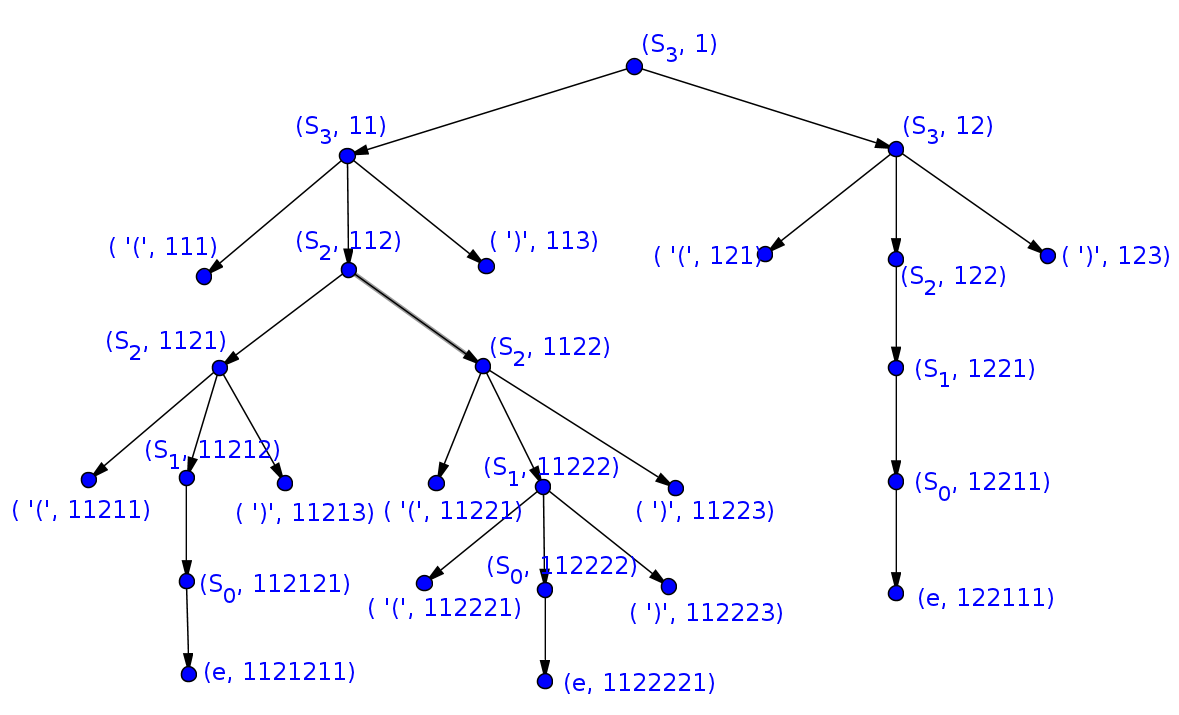
\includegraphics[width = \textwidth]{tree-1.png}}

\smallskip

{\bf (iv-a).} Слово $\eps$ имеет два различных вывода, показанных в задаче 3. При построенние деревья получатся разными. 

\end{document}
